%%%%%%%%%%%%%%%%%%%%%%%
%%      Lecon 4      %%
%%%%%%%%%%%%%%%%%%%%%%%

\chapter{Action, crise des Etats et crise de l'Euro}
\section{Rappel du cercle vicieux}
Voici en 3 images, le résumé de la situation expliquée dans les chapitres précédents. Je trouve que les schémas sont bien faits et ne nécéssite pas d'explication supplémentaires.\\
 
\begin{minipage}{0.5\textwidth}
	\begin{flushleft}
		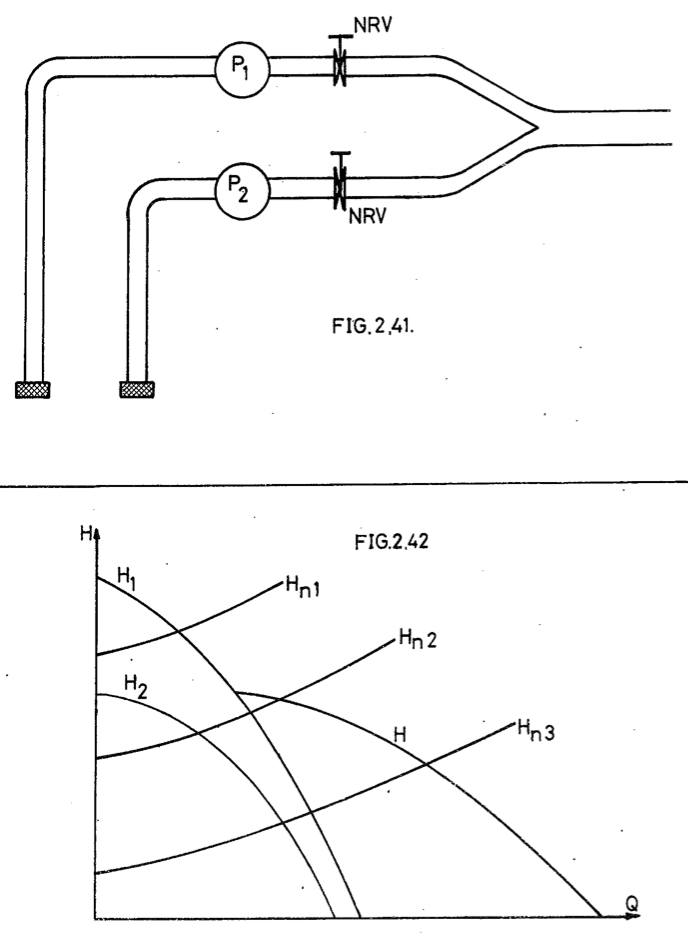
\includegraphics[scale=0.26]{27}
	\end{flushleft}
\end{minipage}
\begin{minipage}{0.5\textwidth}
	\begin{center}
		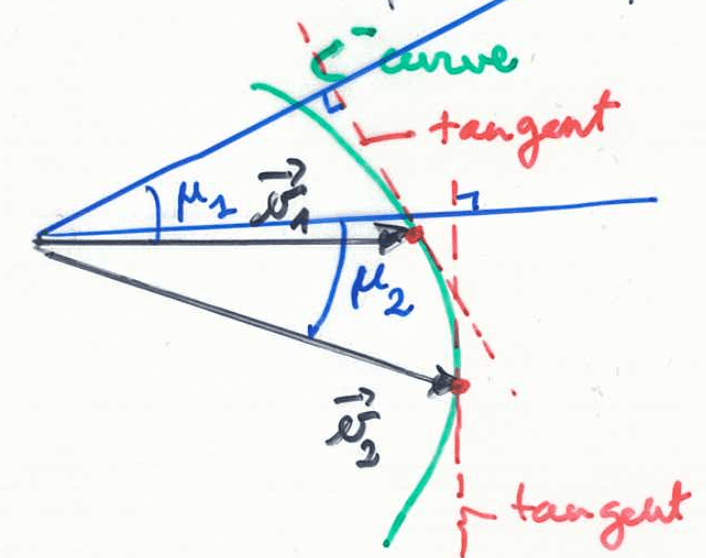
\includegraphics[scale=0.26]{28}
	\end{center}
\end{minipage}
\ \\
\begin{center}
	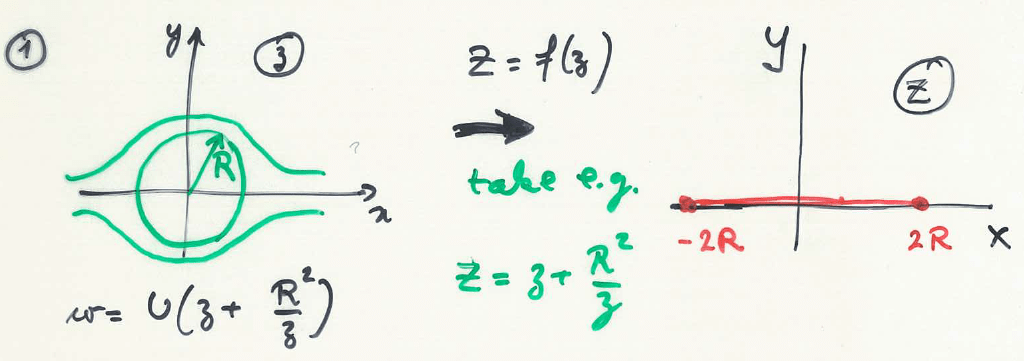
\includegraphics[scale=0.3]{29}
\end{center}

\section{Construction de l'Europe}
\subsection{Le début}

\begin{itemize}
	\item \textbf{1948 - 1952, les fondements intellectuels :} \\ 
	      On vient de sortir d'une grande guerre et il faut rebâtir l'Europe. Schuman, Adenauer et Monnet commencent à réfléchir à une union.
	      	
	\item \textbf{1952, Communauté Européenne du Charbon et de l'Acier :} \\
	      Il faut relancer l'industrie européenne. 6 pays décident de créer une alliance économique et non militaire : All, Fr, It et Benelux. On élargira la coopération à Euratom (nucléaire) par la suite.
	      	
	\item \textbf{1957-1958, Traité de Rome :} \\
	      La CECA s'élargie à la Communauté Economique Européenne qui devient donc un marché commun (suppression progressive des frontière) et dont l'éxécutif est la Commission Européenne. La coopération de l'Allemagne et de la France crée un axe très solide. 
\end{itemize}

\subsection{Un long chemin}
On a du parcourir un long chemin, avant d'en arriver à l'union d'aujourd'hui. Dans les grandes lignes, on a eu :

\begin{itemize}
	\item \textbf{De nombreux échecs :} \\
	      En 1953, la création d'une Communauté Européenne de Défense a échoué. En 1965 et 1967, la France pose son véto à l'entrée de la Grande Bretagne dans l'union. Et en 1970, les nombreuses tentatives de monnaie unique ont échouées.
	      	
	\item \textbf{Des élargissements successifs :} \\
	      Aux 6 pays créateurs se sont ajoutés, le UK, le Dannemark et l'Irlande en 1973, la Grèce qui était passé à la démocratie en 1981 et l'Espagne et le Portugal qui sont également des démocraties mais qui sont également de grands concurrents agricoles pour les pays membres, en 1986.
	      	
	\item \textbf{Des approfondissements financiers :} \\
	      On créa, en 1979, le Système monétaire Européen (SME) qui se chargeait des fluctuations des différentes monnaies présentes dans l'union pour avoir des devises assez liées. 
	      	
	\item \textbf{Mais aussi démocratiques :} \\
	      On éli les membres pour le Parlement européen pour la première fois en 1979 et on signe le Traité de Schengen de libre circulation en 1985.
\end{itemize}

\subsection{Le grand bond en avant}
Cette union a eu énormement de succès, dont :

\begin{itemize}
	\item \textbf{1989, chute du mur de Berlin :} \\
	      Celle-ci partageait l'Allemagne en deux et seul la partie ouest faisait partie de l'union. L'intégration de cette partie directement posait problème aux Français puisque l'Allemagne allait gagné en voix. Cependant, les Français acceptait l'intégration de la partie Est si l'Allemagne était d'accord d'adopter l'Euro. 
	      	
	\item \textbf{1992, Traité de Maastricht :} \\
	      On signe ici une union politique qui donne à l'Union Européennne des compétences étatiques et on forge une union monétaire, l'Euro. 
	      	
	\item \textbf{Les Etats abandonnent des compétences souveraines :} \\
	      Comme émettre la monnaie, la politique judiciaire, de police, pénale et la politique de sécurité extérieure (ex : instabilité en ex-Yugoslavie).
	      
	\item \textbf{1995, Suède, Autriche, Finlande :} \\
	      L'intégration de ces pays a été rendu possible par la fin du communisme. 
	      	
	\item \textbf{2004, ex pays de l'est et Méditerrannée :} \\
	      On intègre la Slovénie, Slovaquie, Tchéquie, Pologne, Hongrie, les Pays Baltes, Malte et Chypre.
	      	
	\item \textbf{2007, Roumanie et Bulgarie.}
	      	
	\item \textbf{2013, Croatie.}
	      	
	\item \textbf{Pour le futur :}
	      L'Europe attire toujours la Serbie, Montenegro, Macédoine, Albanie et la Turquie.
\end{itemize}

\section{L'Union Monétaire et l'Euro}
\subsection{Le difficile traîté de Maastricht}
Quelles étaient les éxigences des pays face à une union monétaire ? Ils voulaient avoir une évolution économique parallèle avec, notamment, la même croissance, inflation, coût salarial et la même compétitivité sur le marché, mais aussi un contrôle sur les déficits.\\
On voulait également avoir des économies qui ne réagissent pas trop différemment aux chocs économiques pour garder ce parallélisme. \\
Ce n'est pas tout. On voulait avoir des mécanismes aptes à remédier aux écarts entre les pays, comme prendre des décisions d'états coordonnées, contrôler l'évolution des salaires et des prix, mais aussi avoir une bonne politique de migration des travailleurs et des capitaux. 

\subsection{Les risques}
Cependant, il y avait certains problèmes. Tout d'abord, les pays du centre étaient bien plus industrialisés que les pays de la périphérie, ce qui provoquait une divergence économique. De plus, la cohérence politique sur certains points est incertaine. Malgrés cela, il fallait adopter cette monnaie commune en raison des taux de change flottants qui conduisent à de l'instabilité, la mondialisation, la libralisation de la circulation des capitaux (risqué car fait fluctué la monnaie) et la volonté des acteurs principaux en Europe. \\
Cependant, on a signé un \textbf{pacte de stabilité} qui limite le déficit public et impose la supervision de la Commission Européenne. On veut aller plus loin dans la coopération en autorisant les réformes structurelles dans la compétitivité, pensions et l'intégration politique.

\subsection{Naissance et élargissements de l'Euro}
Malgré toutes les difficultés, 11 Etats choisissent l'adoption de la monnaie commune. En 1999,, les marchés financiers adoptent donc l'euro (marché des changes, la bourse, la dette publique, les trésoreries des entreprises). Et dès le 1er jannvier 2002, on utilise la nouvelle monnaie. \\
Il y a eu des élargissement par la suite. Entrent dans l'euro, la Grèce en 2001, la Slovénie, Chypre et Malte, Slovaquie, Estonie et en 2014 la Lituanie. On décide que tous les nouveaux pays adhérant à l'UE doivent adopter l'euro quand les conditions sont remplies. 

\section{Cohésion à l'épreuve}

\begin{wrapfigure}[7]{l}{8cm}
	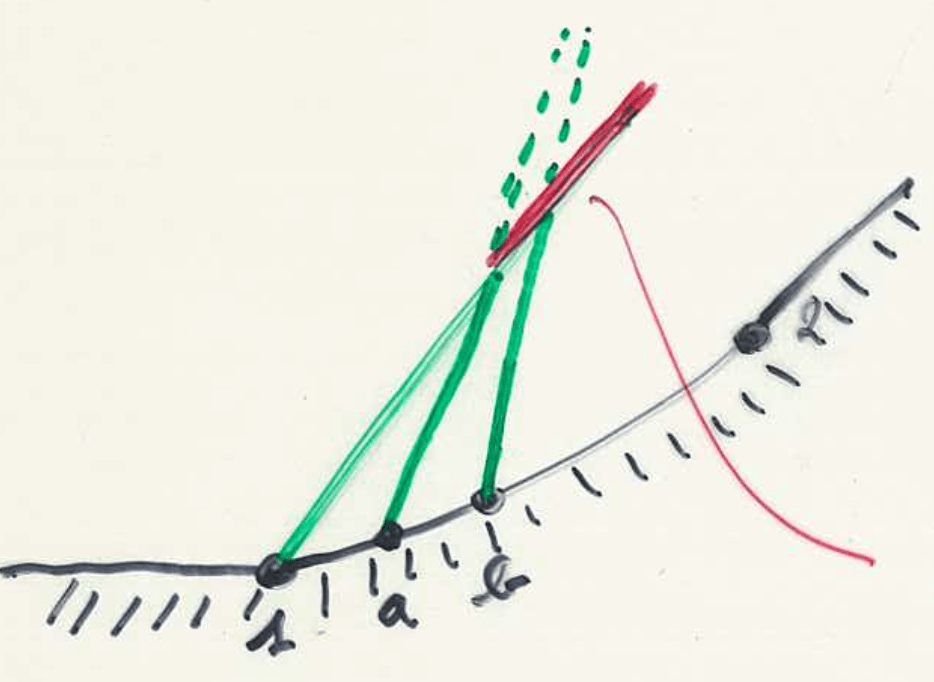
\includegraphics[scale=0.3]{30}
\end{wrapfigure}
\noindent Par contre, ça ne va pas très bien dans la zone euro. On avait dit qu'on ne voulait pas de disparité au niveau de la croissance des Etats mais c'est tout le contraire qui se passe ici. Les "grands pays" subissent une décroissance de leur PIB alors que les pays les plus à l'est tire profit de la nouvelle alliance. \\\\\\

\begin{wrapfigure}[7]{l}{8cm}
	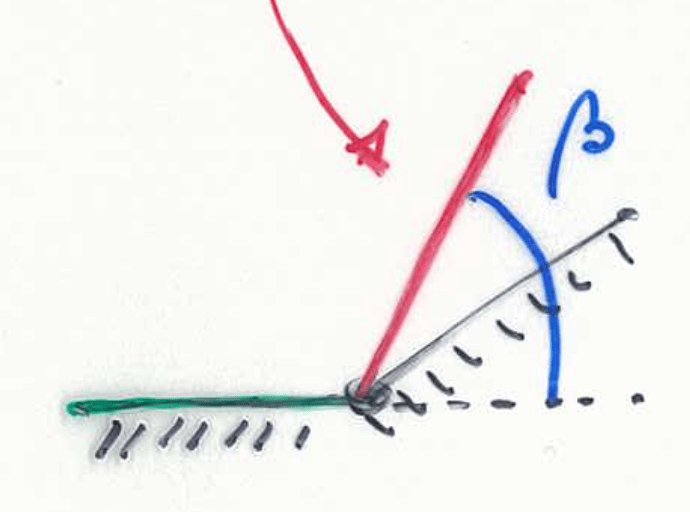
\includegraphics[scale=0.3]{31}
\end{wrapfigure}
\noindent Ceci est en grande partie dû à la forte montée du chômage au sein de la zone euro qui atteint les 20\% en Espagne et Lettonie. La Lettonie est d'ailleurs le pays le plus touché d'après le graphique précédent. De nouveau, les chiffres sont très différents d'un pays à l'autre. C'est le deuxième élément de divergence. \\\\\\

\begin{wrapfigure}[11]{l}{8.5cm}
	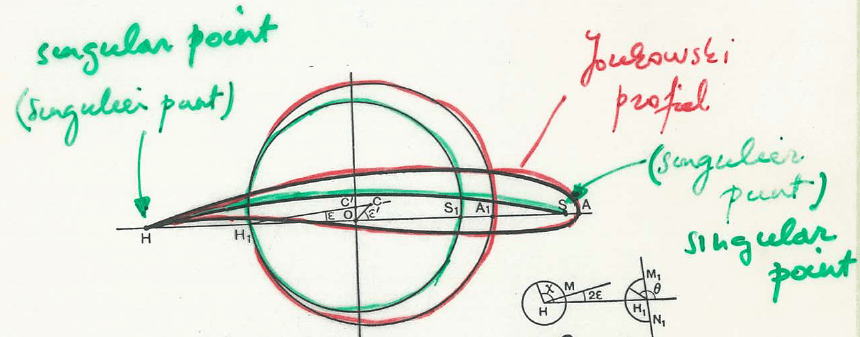
\includegraphics[scale=0.3]{32}
\end{wrapfigure}
\noindent Le troisième élément de divergence est la différence que l'on rencontre dans les déficits. En effet, selon le graphique, on peut voir un mouvement d'ensemble pour certains pays mais également d'autres pays comme l'Irlande qui ne suivent plus du tout la cohésion. Le déficit de l'Irlande atteint d'ailleurs les 25\% ce qui est un grand signe d'instabilité. \\\\\\\\

La très forte pression sur le budget des Etats (en raison de l'aide aux banques) va faire qu'à un moment, le budget ne supporte plus. Ceci fait monter l'austérité et influence l'économie globale qui se porte de plus en plus mal. Ceci met les Etats encore plus en difficulté  et sont forcés de couper certaines aides aux banques. Ceci mécontente les banques et instabilise totalement l'économie. Les Etats sont, dès lors, obligés de s'endetter.

\begin{wrapfigure}[11]{l}{9cm}
	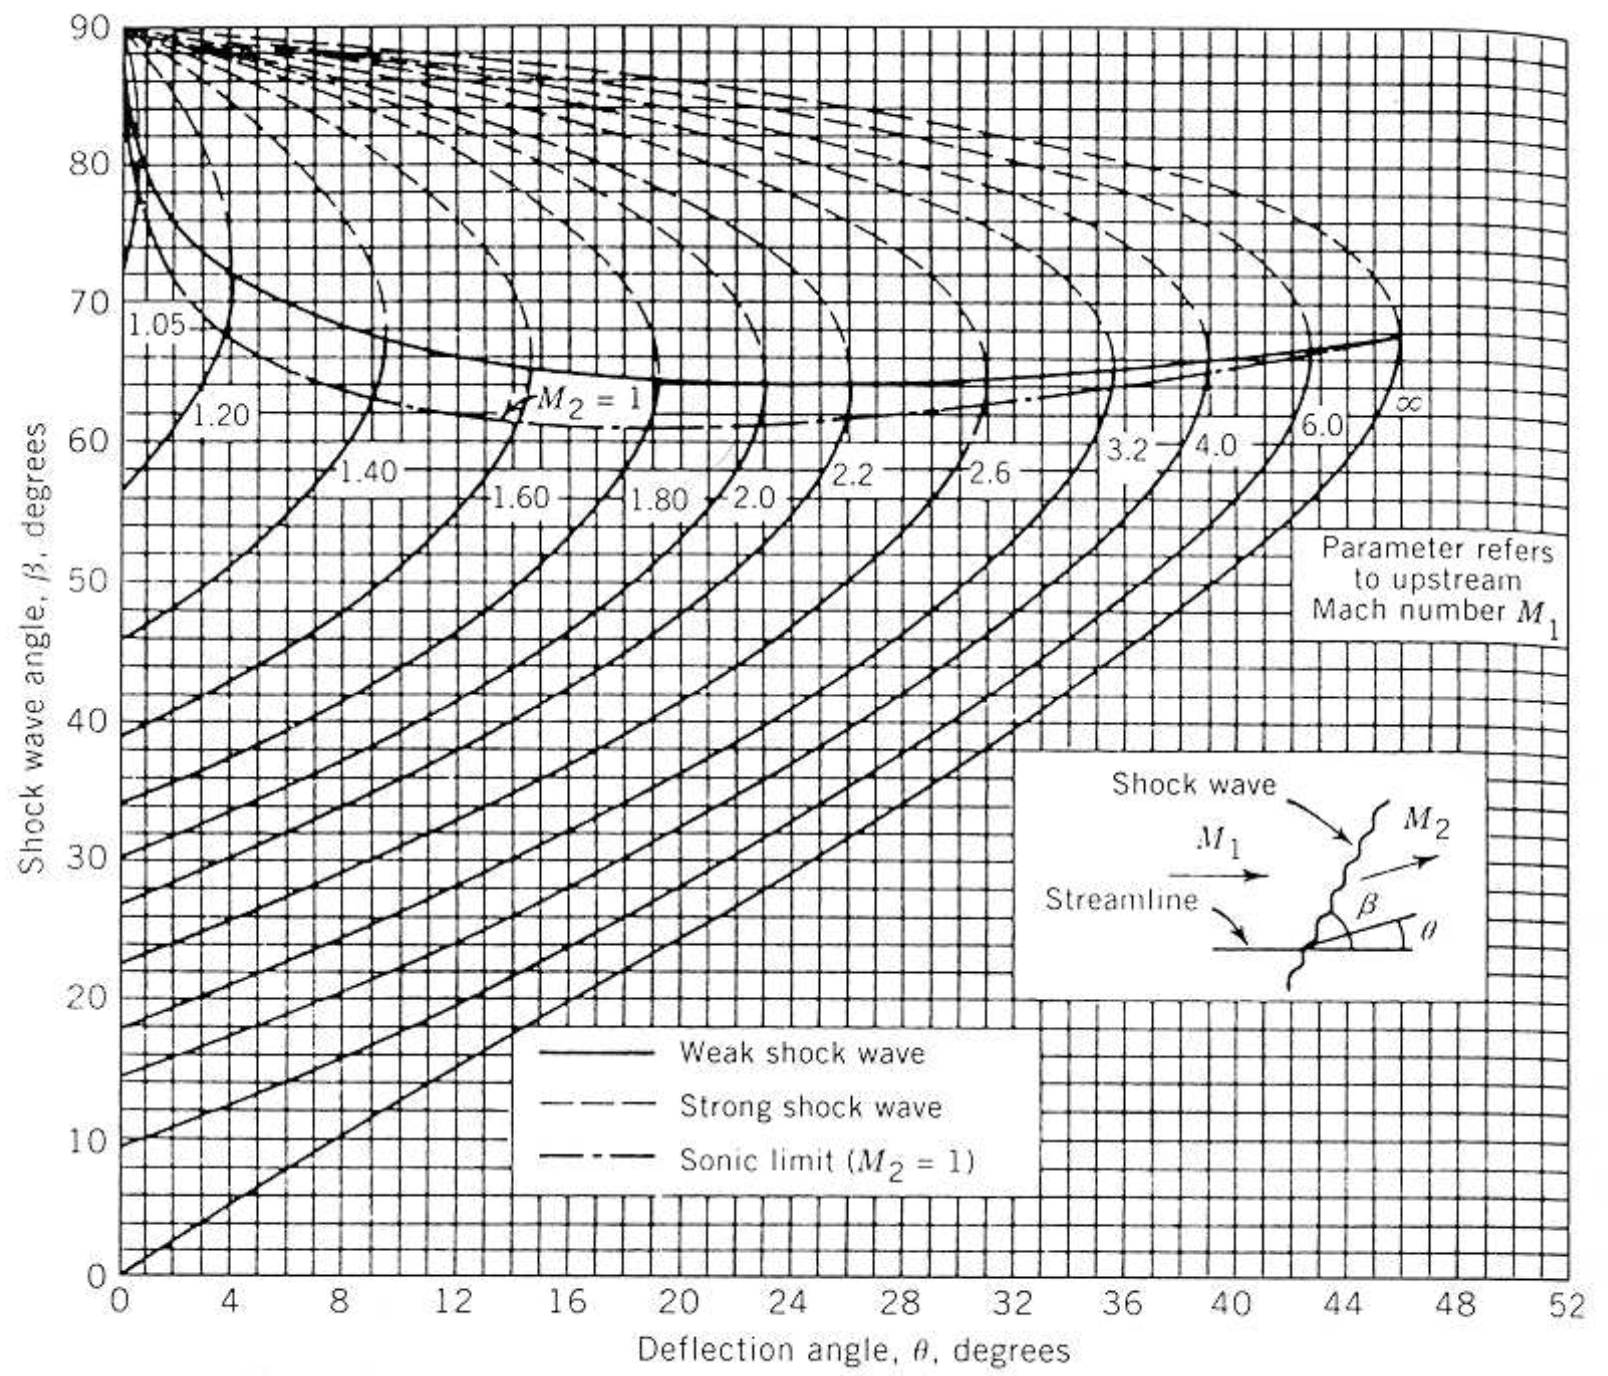
\includegraphics[scale=0.3]{36}
\end{wrapfigure}
\ \\ \\ La dernière et la plus importante des divergence s'observe au niveau des dettes publiques. Le graphe montre très bien ce phénomène et met en avant un problème majeur : la dette de la Grèce qui a atteint les 175\% de sont PIB. Beaucoup d'autres pays sont au dessus des 100\% de dette, ce qui traduit également une inefficacité de l'union.

\section{Situation de la Grèce}
\subsection{L'entrée dans l'euro}
Les critères à valider pour entrer dans l'euro sont : avoir un déficit des finances public inférieur à 3\% du PIB et la dette public doit être inférieur à 6\% ou doit diminuer chaque année. Jusqu'en 1994, la dette de la Grèce reste supérieur à 10\% donc ne sait pas entrer dans l'euro. Mais elle annonce en 1999 que son déficit est en dessous des 3\% donc peut entrer dans la zone euro en 2000. Elle doit maintenant pouvoir maintenanir ces 3\% et pour ça, elle va faire preuve de "créativité" économique et va utiliser, dès 2001, des instruments financiers qui permettent de cacher une partie de la dette. \\
Cependant, à partir de 2002, les doutes commencent à se réveiller car il y a un changement à partir de 2000 sur les données de la Grèce. On a des difficultés à voir clair. Les doutes commencent aussi pour d'autres pays comme l'Italie et le Portugal. 

\subsection{Première alerte en 2005}
Eurostat refuse de valider les chiffres grecs ! Ceci survient juste avant les élections mais le nouveau gouvernement va entreprendre des audits approndie afin de résoudre cette énigme. Celui-ci révèle des déficits bien plus élevés que ceux déclarer !\\
De ce fait, la Comission Européenne ouvre les procédure d'infraction contre la Grèce car le déficit est supérieur à 3\%. Mais pas seulement en Grèce. En Italie, Allemagne, France et Portugal aussi. Néanmoins, la Grèce réussi quand même à ramener son déficit à 2.6\% en 2006 (contre 5.5\% en 2005) donc tout va bien.

\begin{wrapfigure}[10]{l}{9cm}
	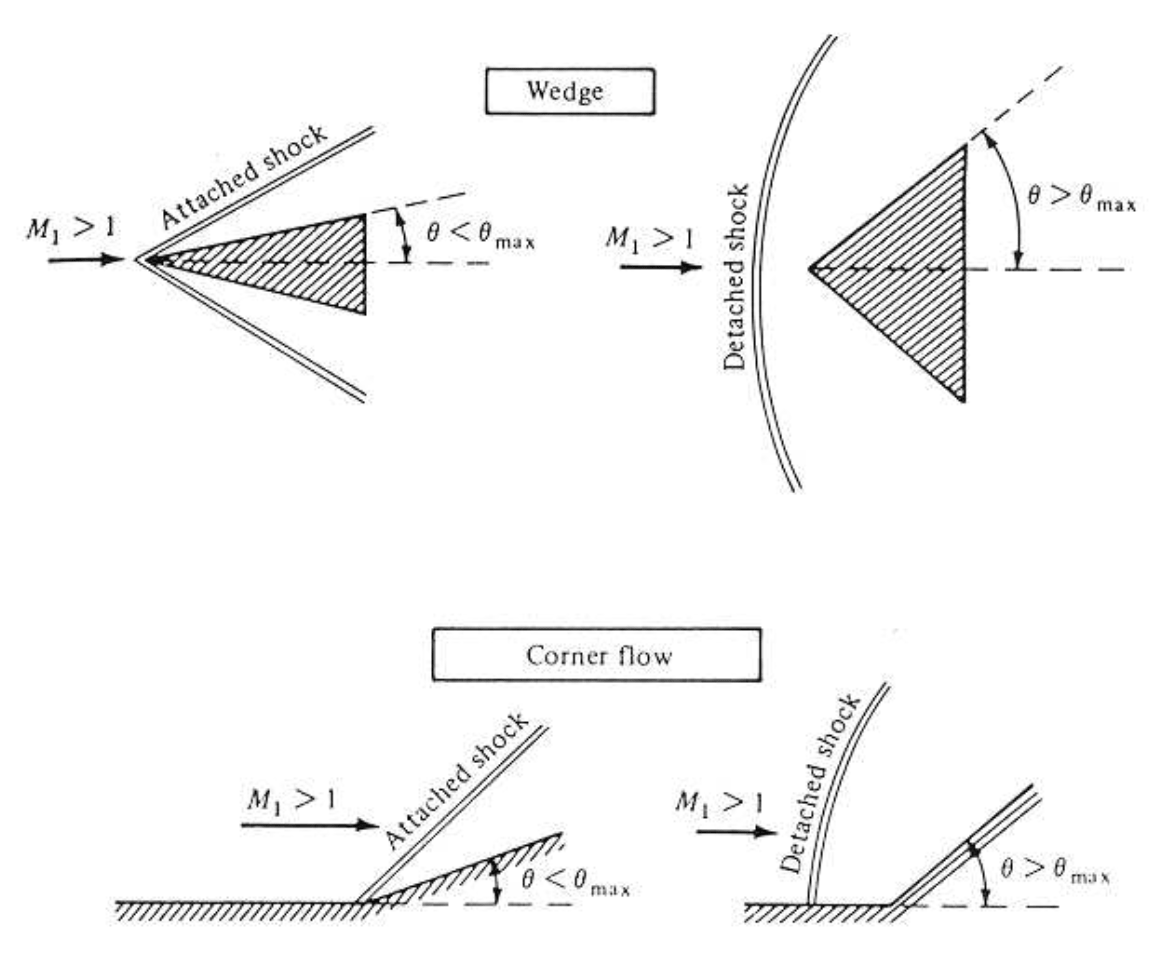
\includegraphics[scale=0.3]{37}
\end{wrapfigure}
\ \\\\On décide en 2009 de faire une révision des chiffres. C'est ici que la vérité est découverte. Les chiffres sont bien plus élevés que ce que les Grecs ont déclarés. Si on ajoute à cela l'épisode de la crise en 2007, la situation s'aggrave et la confiance accordée au pays est fortement perturbée. Les conséquences sont :

\begin{enumerate}
	\item La « notation »\footnote{C'est l'apréciation donnée (note de confiance) par une agence à un pays. Cela permet de connaître les pays à risque et ceux où il est bon d'investir.} de la dette grecque est dégradée de A à BBB+ le 16 décembre 2009
	      
	\item Les capitaux fuient le pays vers d'autres où ils seront en sécurité.
	      	
	\item Les taux d’intérêt grecs augmentent.
\end{enumerate}   

\begin{wrapfigure}[9]{l}{9cm}
	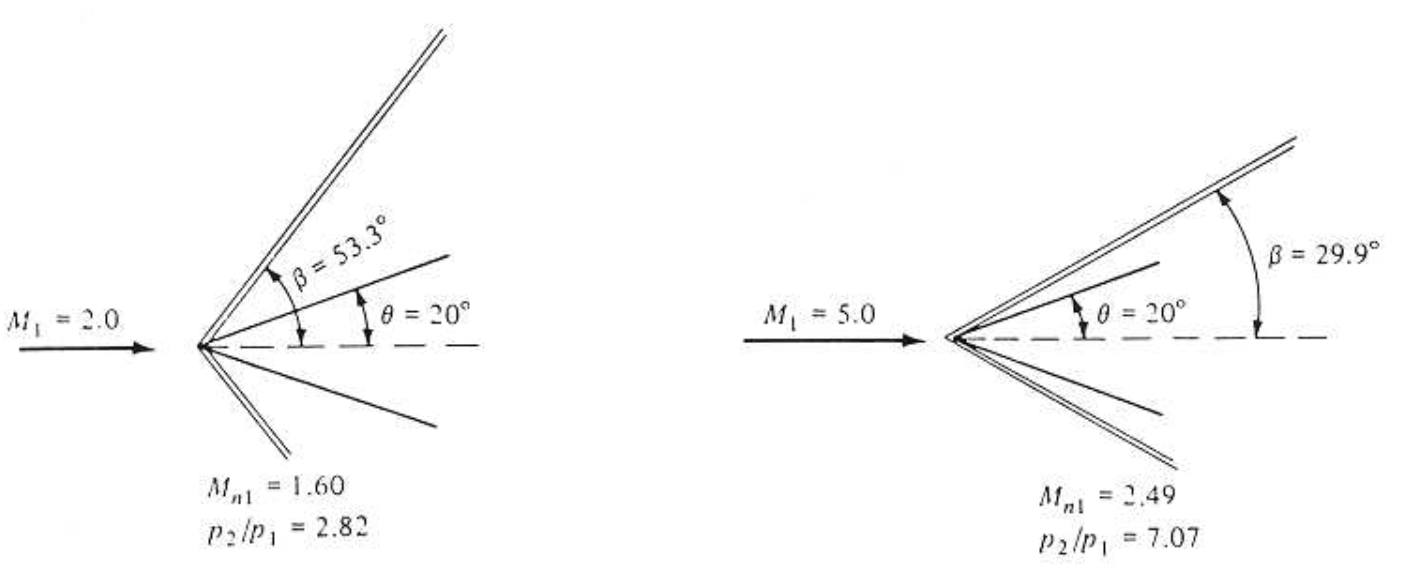
\includegraphics[scale=0.3]{38}
\end{wrapfigure}
\ \\ Une des conséquences majeures est que le taux d'intérêt reste assez élevé comparé aux autres pays. Ceci est en partie dû à la perte de confiance et la difficulté de remboursement des prêts. Il faut apporter un soutien rapidement pour remédier à cette situation. \\\\\\\\

\subsection{Plan de sauvetage}
Le gouvernement grec adopte un plan de réduction drastique du déficit (dépenses militaires, hopitaux, retraite, gel du nombre de fonctionnaire et baisse des salaires) et diminue ses dépenses de 52.0\% à 50.6\% du PIB de 2009 à 2010. \\
Le gouvernement relève les recettes du pays de 39,3\% à 41,9\% du PIB de 2009 à 2010 grâce à une réduction de la fraude fiscale, des taxes supplémentaires, impôts sur les entreprise et l'immobilier et hausse de la TVA.\\
Par ailleurs, l'Europe avait promis une aide financière. Mais la pression sur les marchés ne diminue pas ! Le 23 avril 2010, la Grèce demande l'aide du FMI et de l'EU.\\
L'EU appelle à la solidarité financière pour assurer la survie de l’euro. Pas seulement pour la Grèce mais aussi pour l’Espagne et le Portugal (voire l'Italie). On prépare des fonds de stabilisation de 750 Milliards d'euros dont 60 milliards empruntés par la Commission européenne, 440 milliards euros apportés par les Etats européens (Belgique : 15 puis de 27 milliards) et 250 milliards euros apportés par le FMI. On prête à la Grèce de 110 Milliards d'euros, soit 10.000 euros par grec ! Cependant la pression des marchés financiers ne va pas s’arrêter. Les gestionnaires de fonds continuent à quitter la Grèce et à investir dans les pays sûrs.

\subsection{Résultat du plan de sauvetage}
\begin{wrapfigure}[12]{l}{9cm}
	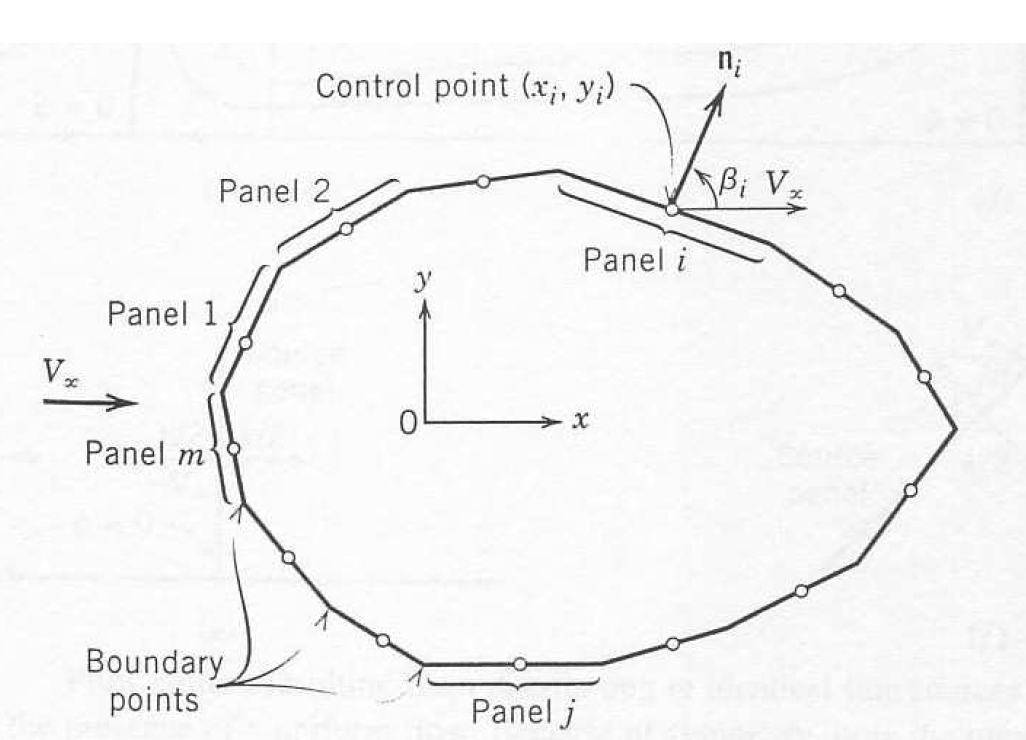
\includegraphics[scale=0.3]{39}
\end{wrapfigure}
\noindent On est dans une véritable crise de gouvernance. L'aide est tardive et le résultat est décevant. Comme on peut le constater, le taux d'intérêt de la dette de la Grèce ne cesse d'augmenter et est exhorbitante par rapport à celui de l'Allemagne. Pour ce qui est de l'évolution annuelle du PIB, elle décroche en 2009 et ne cesse de diminuer (-8.9\% en 2011). Pareil pour le PIB/habitants, elle descend de 63\% de celle des Belges à 50\% (diapos 10-13 pour les graphiques).\\
Nous sommes dans une impasse (mai 2011) parce que la Grèce n’est plus capable d’emprunter, la population grecque s'oppose progressivement à l‘austérité et donc on ne sait plus mettre en place des réformes fiscales structurelles. Petit à petit, les pays européens se divisent. Doit-on faire payer les emprunteurs seulement ou les prêteurs aussi ?\\
De juillet à Octobre 2011 ont lieu des négociations intenses. On décide d'accélérer l’intervention internationale de 110 milliards euros et d'abandonner une dette de 50 milliards (par les banques privées nationales et internationales). L’essentiel de la dette grecque est dorénavant détenu par les autres états. Malgré cela, le plan de réformes (austérité) doit être poursuivi.

\begin{wrapfigure}[13]{l}{9cm}
	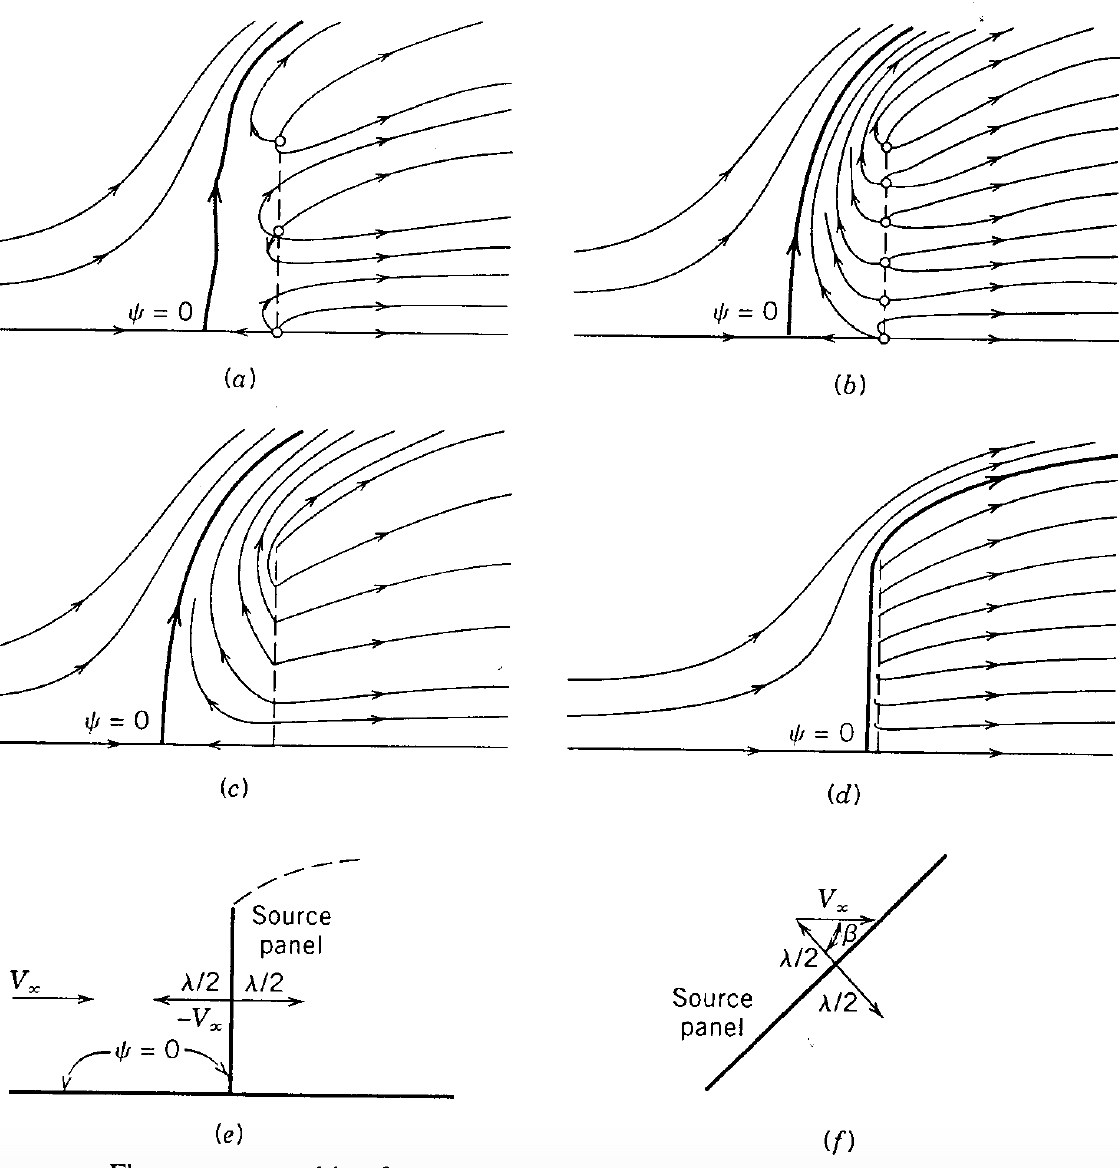
\includegraphics[scale=0.3]{40}
\end{wrapfigure}
\ \\ On voit que les grandes décisions prises en 2011 ont fortement contribué à la réduction du taux d'intérêt. Néanmoins, cela reste insuffisant et de nouvelles actions de solidarité doivent être mené en Grèce, Irlande, Portugalet Espagne. Mais les opignons publiques rejettent les plans d'austérité et entraine des conséquences potiques (montée du nationalisme, protectionnisme, repli sur soi, populisme anti-européen). On observe aussi la montée des extrêmes en Italie (élections de février 2013) et en Grèce (élections de janvier 2015). \\
D'autre part, la solidarité financière est rejetée par les opinions publiques des
pays « riches » (Allemagne, Finlande, Pays-Bas, et même France) ce qui provoque une faiblesse institutionnelle de l’Union européenne.

\subsection{Deux visions sur la crise greque}
Voici les deux slides qui reprennent assez bien les deux opignons. La première présente les causes et la deuxième, les solutions. 

\begin{center}
	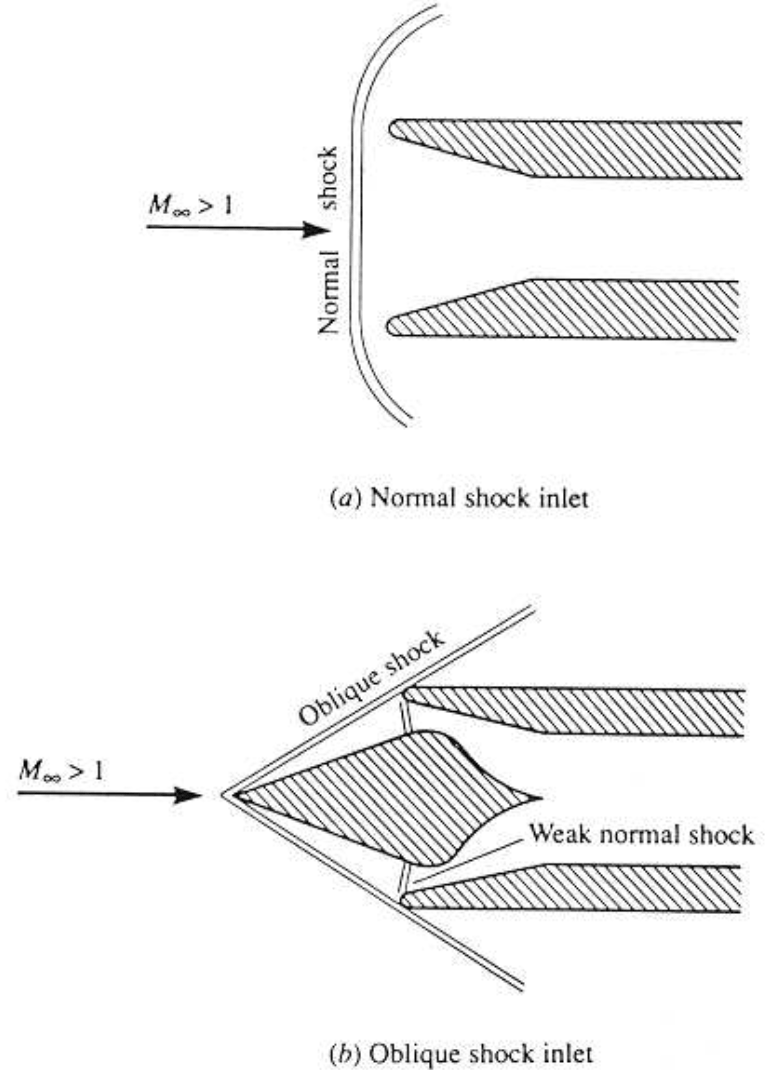
\includegraphics[scale=0.5]{41}
\end{center}

\begin{center}
	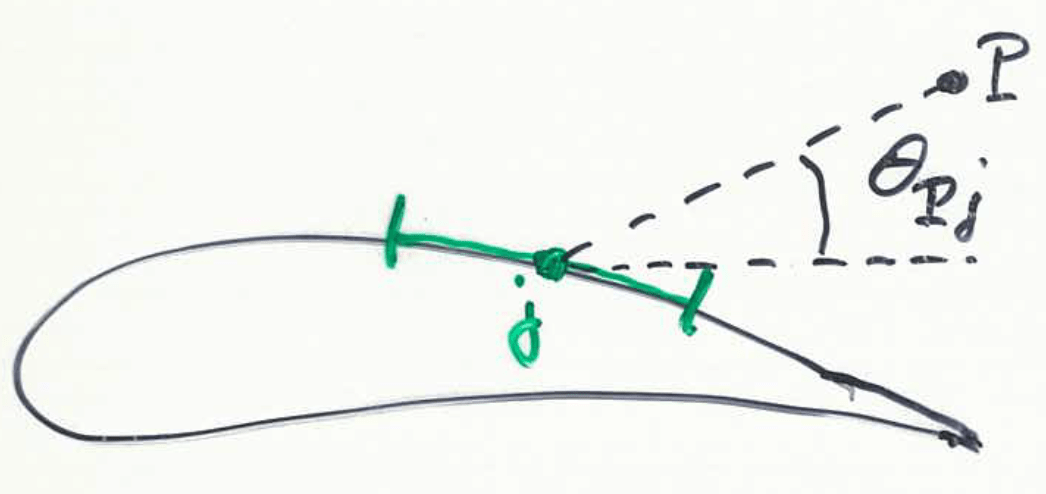
\includegraphics[scale=0.5]{42}
\end{center}